%%%%%%%%%%%%%%%%%%%% book.tex %%%%%%%%%%%%%%%%%%%%%%%%%%%%%
%
% sample root file for the chapters of your "monograph"
%
% Use this file as a template for your own input.
%
%%%%%%%%%%%%%%%% Springer-Verlag %%%%%%%%%%%%%%%%%%%%%%%%%%


% RECOMMENDED %%%%%%%%%%%%%%%%%%%%%%%%%%%%%%%%%%%%%%%%%%%%%%%%%%%
\documentclass[envcountsame,envcountchap]{svmono}

% choose options for [] as required from the list
% in the Reference Guide, Sect. 2.2
\usepackage[cmex10]{amsmath}
\usepackage{makeidx}         % allows index generation
\usepackage{graphicx}        % standard LaTeX graphics tool
                             % when including figure files
\usepackage{multicol}        % used for the two-column index
\usepackage[bottom]{footmisc}% places footnotes at page bottom
% etc.
% see the list of further useful packages
% in the Reference Guide, Sects. 2.3, 3.1-3.3

\makeindex             % used for the subject index
                       % please use the style svind.ist with
                       % your makeindex program


%%%%%%%%%%%%%%%%%%%%%%%%%%%%%%%%%%%%%%%%%%%%%%%%%%%%%%%%%%%%%%%%%%%%%

\begin{document}

\author{Ubon Thongsatapornwatana\\ Chanatip Chuenmanus}
\title{Suspect Vehicle Detection using Vehicle Reputation with Association Analysis Concept\\
%{\small SPIN Springer's internal project number, if known}
}
\subtitle{-- Monograph --}
\maketitle

\frontmatter%%%%%%%%%%%%%%%%%%%%%%%%%%%%%%%%%%%%%%%%%%%%%%%%%%%%%%


%%%%%%%%%%%%%%%%%%%%%%% dedic.tex %%%%%%%%%%%%%%%%%%%%%%%%%%%%%%%%%
%
% sample dedication
%
% Use this file as a template for your own input.
%
%%%%%%%%%%%%%%%%%%%%%%%% Springer-Verlag %%%%%%%%%%%%%%%%%%%%%%%%%%

\thispagestyle{empty}
\vspace*{3.5cm}
\begin{flushright}

% write your text here
{\large Your dedication goes here}

\end{flushright}




%%%%%%%%%%%%%%%%%%%%%% pref.tex %%%%%%%%%%%%%%%%%%%%%%%%%%%%%%%%%%%%%
%
% sample preface
%
% Use this file as a template for your own input.
%
%%%%%%%%%%%%%%%%%%%%%%%% Springer-Verlag %%%%%%%%%%%%%%%%%%%%%%%%%%

\preface

%% Please write your preface here
Here come the golden words


%% Please "sign" your preface
\vspace{1cm}
\begin{flushright}\noindent
place(s),\hfill {\it First name  Surname}\\
month year\hfill {\it First name  Surname}\\
\end{flushright}




\tableofcontents


\mainmatter%%%%%%%%%%%%%%%%%%%%%%%%%%%%%%%%%%%%%%%%%%%%%%%%%%%%%%%
%%%%%%%%%%%%%%%%%%%%%%%% part.tex %%%%%%%%%%%%%%%%%%%%%%%%%%%%%%%%%%
%
% sample part title
%
% Use this file as a template for your own input.
%
%%%%%%%%%%%%%%%%%%%%%%%% Springer-Verlag %%%%%%%%%%%%%%%%%%%%%%%%%%


\part{Part Title}

%%%%%%%%%%%%%%%%%%%%% chapter.tex %%%%%%%%%%%%%%%%%%%%%%%%%%%%%%%%%
%
% sample chapter
%
% Use this file as a template for your own input.
%
%%%%%%%%%%%%%%%%%%%%%%%% Springer-Verlag %%%%%%%%%%%%%%%%%%%%%%%%%%

\chapter{Suspect Vehicle Detection using Vehicle Reputation with Association Analysis Concept}
\label{intro} % Always give a unique label
% use \chaptermark{}
% to alter or adjust the chapter heading in the running head

The suspect vehicle detection system normally compares the list of criminal license plates and vehicle license plates gathering from various sensors in order to identify the criminal vehicles or the suspect vehicles. 
However, the traditional process of comparing those license plates utilizing the matching of alphabet character is not effective. 
If the characters do not match any one character, the system can not detect the criminal vehicles or the suspect vehicles. 
This paper proposes the use of reputation algorithm to detect the criminal vehicles crossing the checkpoint whose license plates match the blacklist. 
In addition to that, we use association analysis concept to detect the suspect vehicles that have ever passed the checkpoint that may be related to the criminal activity records. 
Our method can detect the suspect vehicles with fake license plate by using color, brand and type of the vehicles instead of only the license plate matching to the blacklists.
These two techniques use a blacklist of criminal vehicles and criminal activity recorded in a criminal report database of Defence Technology Institute (DTI), Thailand, to help facilitate the detection process. 
The result shows that the reputation algorithm and the association analysis concept can improve the detection capability of the suspect vehicle detection system.

\section{Introduction}
\label{sec:1}
% Always give a unique label
% and use \ref{<label>} for cross-references
% and \cite{<label>} for bibliographic references
% use \sectionmark{}
% to alter or adjust the section heading in the running head
Reputation concept is a technique to classify object that commonly applied to various systems to make effective automatic detection, such as filtering email spam \cite{DBLP:taylor, lazzari}, vehicle classification \cite{ding,park}, ecommerce \cite{altman,page,resnick}, etc.
In addition, vehicle detection by only data classification process may be insufficient. Therefore, the association analysis process should be used together to increase the detection accuracy.
The traditional suspect vehicle detection process of comparing criminal license plates and vehicle license plates utilizing the matching of alphabet character is not effective. If the characters do not match any one character, the system can not detect criminal or suspect vehicles.

In this paper, we propose the approach using reputation concept to detect criminal vehicles crossing the checkpoint whose license plates match the blacklist. 
In addition, we use association analysis concept to detect the suspect vehicles which license plates do not match the blacklist, however this method uses color, brand and type of vehicles matching the blacklist to identify the vehicles that potentially involve in criminal activity.
The aim of this work is to improve the detection capability of suspect vehicle detection system.

In the next section, we discuss background information and previous studies using reputation algorithm and association analysis concept. Section III explains the research testbed and research design. Experimental results are shown in Section IV, and discussed in Section V. Section VI concludes and presents future directions.

\section{Literature Review}
\label{sec:2}

\subsection{Reputation Algorithm}
\label{sec:3}
The concept of reputation has been used to classify objects in a domain or community. 
An object with a higher reputation score gain more attraction than an object with a lower reputation score.  
Reputation concept has been applied to the several problems in vehicle scoring system.  
It works well for filtering false messages in vehicular ad hoc network (VANET) environments \cite{ding} and providing reliable reputation scores for vehicles in VANET initial deployment environment \cite{park}.
The reputation concept is also be applied to other practical applications. For example, Bradley Taylor \cite{DBLP:taylor} uses reputation to classify authenticated sender's domain as either spammy or not spammy within a large webmail service.  Reference \cite{altman} uses the axiomatic approach to deal PageRank, the most famous page ranking algorithm.
We propose the use of this concept to identify criminal vehicles that crossing the checkpoint. 
A high reputation score represents a criminal vehicle, whereas low reputation score represents a normal vehicle.

\subsection{Association Analysis Concept}
\label{sec:4}
Association analysis concept has been widely applied in various systems in previous research.
For example, the concept of mutual information have been used to estimate word association norms between words in English texts \cite{chruch} and to extract a triple of binary strings a, b, c \cite{romashchenko}.
Reference \cite{kaza} used association analysis by using the concept of mutual information measurement to identify potentially target vehicles that cross the border frequently with the vehicles which are involved in criminal activity.
Association analysis by using the idea of association rule has also been used to analyze frequent access crunode extracted from previous sequences \cite{li} and to extract valuable industrial data from massive data storage \cite{zhuang}.
G. Miao et al. \cite{miao} used a new ranking algorithm, based on Latent Association Analysis (LAA) by considering
the semantic associations among document pairs to rank target documents using the latent factor.

\section{Research Testbed and Design}
\label{sec:5}

\subsection{Research Testbed}
\label{sec:6}
The testbed for this research includes the blacklist of the criminal vehicle data set and the criminal activity data set obtained from criminal report database of Defence Technology Institute (DTI), Thailand.
Moreover, this testbed consists of the lists of the checkpoint crossing data set from various sensors includes the license plate, vehicle brand, vehicle color, vehicle type, checkpoint, crossing date and time. The checkpoint crossing data set is divided into two categories: 1) The one year records. 2) The real time checkpoint crossing records in three months. Details of these data sets are shown in Table \ref{table_inputData}.

\begin{table}[!t]
\renewcommand{\arraystretch}{1.2}
\caption{Summary of input data set}
\label{table_inputData}
\centering
\begin{tabular}{c|c}
\hline
\bfseries Input Data Set & \bfseries Summary\\
\hline
Number of the criminal vehicles in blacklist & 4801\\
\hline
Criminal activity records & 1972\\
\hline
The one year checkpoint crossing records & 992017\\
\hline
The real time checkpoint crossing records in three months & 281089\\
\hline
Number of the vehicles crossing the checkpoint in three months& 90563\\
\hline
Number of criminal vehicles crossing the checkpoint in three months& 513\\
\hline
\end{tabular}
\end{table}

\subsection{Research Design}
\label{sec:7}

\begin{figure*}
\centering
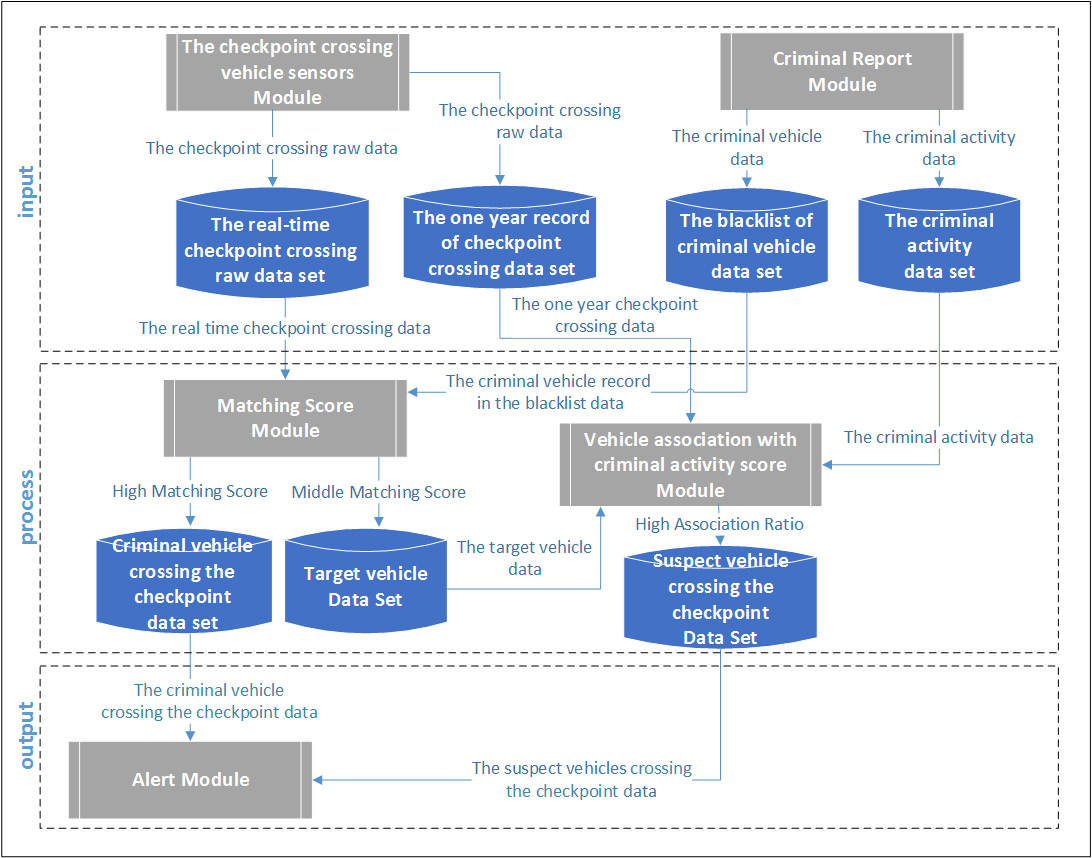
\includegraphics[width=1\textwidth]{images/myfigure.jpg}
\caption{Research design and process diagram.}
\label{fig:diagram}
\end{figure*}

Fig. \ref{fig:diagram} shows the research design and the evolution process of criminal or suspect vehicle detection at the checkpoint. This diagram is divided into three sections: 
1) Input section consists of the real time checkpoint crossing data set in three months, the one year records of checkpoint crossing data set, the blacklist of criminal vehicle data set, and criminal activity data set. 
2) Processing section consists of matching score module to detect the criminal vehicles that crossing the checkpoint and vehicle association with criminal activity score module to detect the suspect vehicles that crossing the checkpoint. In this research, we focus on the processing section shown in Fig.\ref{fig:diagram} which is explained in the following sub-sections. 
3) Output section serves as the alert of the criminal vehicle or suspect vehicle if the system detects the criminal vehicles or suspect vehicles that crossing the checkpoint. 

\subsubsection{Matching Score Module}
Matching Score Module is criminal vehicle detection process. 
First, we define attributes for classification and assign weight to each of the attributes. 
Higher weight is assigned to higher significant attributes.
In this research, we select the license plate, vehicle color, vehicle brand, and vehicle type to be used in the classification and we assign higher weight to license plate than vehicle color, vehicle brand, and vehicle type. 
The system compares the real time checkpoint crossing records in three months and criminal vehicle records in the blacklist by using following attributes: license plate, vehicle color, vehicle brand, and vehicle type. 
Subsequently, it computes the sum of all of the weighted attribute. 
The weighted sum is a single number to compare with the threshold.  
If weighted sum is greater than the high score threshold, referred to as “High Matching Score”, vehicle crossing the checkpoint will be considered as criminal vehicle and will be processed in the Alert Module. 
If weighted sum is less than the high score threshold and also greater than the low score threshold, referred to as “Middle Matching Score”, vehicle crossing the checkpoint will be considered as target vehicle and will be processed in the Vehicle Association with Criminal Activity Score Module. 

High Matching Score is calculated by the following attribute-matching condition: at least license plate matches with the blacklist.
Middle Matching Score is calculated by the following attribute-matching condition: vehicle color and vehicle brand and vehicle type match with the blacklist. 
Algorithm of Matching Score Module is shown in Fig. \ref{fig:matchingAlgo}. Table \ref{table_variableMatching} summarizes the notation for Matching Score Module.

\begin{figure}
\centering
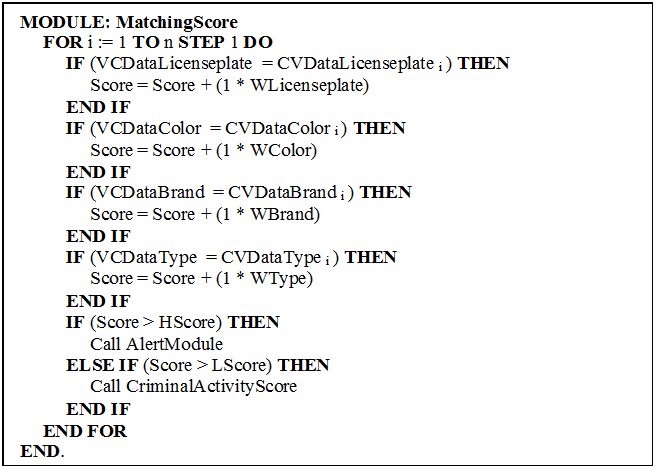
\includegraphics[width=1\textwidth]{images/MatchingAlgorithm.jpg}
\caption{Matching score module algorithm.}
\label{fig:matchingAlgo}
\end{figure}

%put these in Notation table
\begin{table}[!t]
\renewcommand{\arraystretch}{1.2}
\caption{Variable Description for Matching Score Module}
\label{table_variableMatching}
\centering
\begin{tabular}{c|l}
\hline
\bfseries Variables & \multicolumn{1}{c}{\bfseries Description}\\
\hline
VCDataLicenseplate & The license plate of vehicle that crossing the checkpoint.\\
\hline
VCDataColor & The color of vehicle that crossing the checkpoint.\\
\hline
VCDataBrand & The brand of vehicle that crossing the checkpoint.\\
\hline
VCDataType & The type of vehicle that crossing the checkpoint.\\
\hline
CVDataLicenseplate & The license plate of the criminal vehicle.\\
\hline
CVDataColor & The color of the criminal vehicle.\\
\hline
CVDataBrand & The brand of the criminal vehicle.\\
\hline
CVDataType & The type of the criminal vehicle.\\
\hline
WLicenseplate & The weight of license plate.\\
\hline
WColor & The weight of vehicle color.\\
\hline
WBrand & The weight of vehicle brand.\\
\hline
WType & The weight of vehicle type.\\
\hline
Score & The sum of all of the weighted attribute.\\
\hline
HScore & The high score threshold.\\
\hline
LScore & The low score threshold.\\
\hline
\end{tabular}
\end{table}

\subsubsection{Vehicle Association with Criminal Activity Score Module}
This module is a suspect vehicle detection process using association analysis concept to identify the vehicles that are potentially involved in criminal activities. 
We determine the number of all the one year checkpoint crossing lists of target vehicle by considering the matching of license plate, vehicle color, vehicle brand, and vehicle type. 
Consequently, we analyze the relationship between each of the criminal activity with all the one year checkpoint crossing records of target vehicle, and we further restricted the set to contain only checkpoint crossing records of target vehicle that already crossed the checkpoint near the location, date, and time of criminal activities. 
Such set can be indicated the number of involvement in criminal activities of target vehicle. 
Then we can calculated the association ratio by using in (1) by computing the fraction of number of involvement in criminal activities of target vehicle and number of the checkpoint crossing records of target vehicle to compare with the defined threshold.

\begin{eqnarray} 
\alpha \quad =\quad \frac { \nu  }{ \varsigma  }
\end{eqnarray}
where\mbox{ }\\
$\alpha$ = association ratio. \mbox{ }\\
$\nu$ = number of involvement in criminal activities of target vehicle.\mbox{ }\\
$\varsigma$ = total of the 1 year checkpoint crossing records of target vehicle.

If the vehicles with higher ratio than the threshold, they are considered potential suspect vehicles, and then the vehicle data will be processed in the Alert Module. 
Algorithm of Vehicle association with Criminal Activity Score Module is shown in Fig. \ref{fig:activityAlgo}. Table \ref{table_variableActivity} summarizes the notation for Vehicle Association with Criminal Activity Score Module.

\begin{figure}
\centering
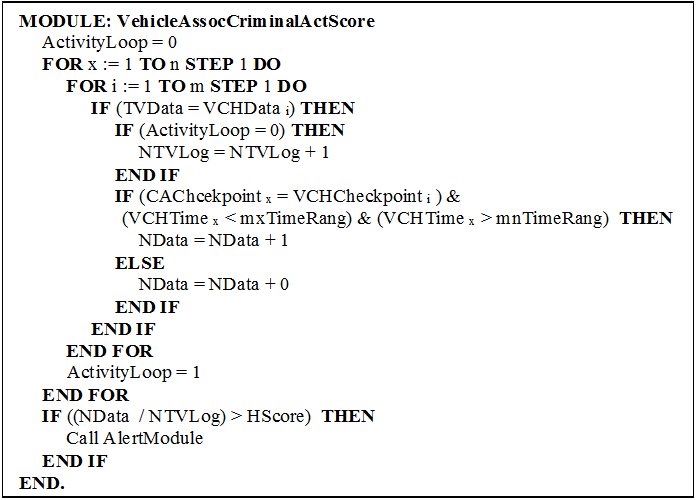
\includegraphics[width=1\textwidth]{images/activityAlgorithm2.jpg}
\caption{Vehicles association with criminal activity score module algorithm.}
\label{fig:activityAlgo}
\end{figure}

\begin{table}[!t]
\renewcommand{\arraystretch}{1.2}
\caption{Variable Description for Vehicle Association with Criminal Activity Score Module}
\label{table_variableActivity}
\centering
\begin{tabular}{c|l}
\hline
\bfseries The Variables & \multicolumn{1}{c}{\bfseries Description}\\
\hline
ActivityLoop & The variable that used to check first iteration in x loop.\\
\hline
TVData & The target vehicle data includes license plate, 
vehicle color, \\ & vehicle brand, and vehicle type.\\
\hline
VCHData & The one year record of checkpoint crossing data set includes  \\ & license plate, vehicle color, vehicle brand, and vehicle type.\\
\hline
NTVLog & Total of one year checkpoint crossing records of target vehicle.\\
\hline
CAChcekpoint & The checkpoint near the location of the criminal activity.\\
\hline
VCHCheckpoint & The checkpoint that target vehicle has ever passed.\\
\hline
VCHTime & Date and time of the checkpoint crossing record.\\
\hline
mxTimeRang & Date and time of the criminal activity plus 1 hour.\\
\hline
mnTimeRang & Date and time of the criminal activity minus 1 hour.\\
\hline
NData & Number of involvement in criminal activities of target vehicle.\\
\hline
HScore & The defined threshold.\\
\hline
\end{tabular}
\end{table}

\section{Experimental Results}
\label{sec:8}
To analyze system performance, there are four factors for analysis as follows:
1) True positive (TP) is the number of the criminal and suspect vehicles that are analyzed as the criminal and suspect vehicles.  
2) True negative (TN) is the number of the normal vehicles that are analyzed as the normal vehicles. 
3) False positive (FP) is the number of the normal vehicles that are analyzed as the criminal and suspect vehicles. 
4) False negative (FN) is the number of the criminal and suspect vehicles that are analyzed as the normal vehicles. 
Such factors can be calculated by using this formula:\\
$$ \text{TP Rate} =  \frac{\text{NofCSVDetectedAsCSV}}{\text{TofCSV}} $$\\
$$ \text{FN Rate} =  \frac{\text{NofCSVDetectedAsNV}}{\text{TofCSV}} $$\\
$$ \text{TN Rate} =  \frac{\text{NofNVDetectedAsNV}}{\text{TofNV}} $$\\ 
$$ \text{FP Rate} =  \frac{\text{NofNVDetectedAsCSV}}{\text{TofNV}} $$\\
$$ \text{Detection Accurate Rate} =  \frac{\text{TP Rate + TN Rate}}{\text{2}} $$

%put this in Notation
\begin{table}[!t]
\renewcommand{\arraystretch}{1.2}
\caption{Variable Description for The System Performance Analysis}
\label{table_variableSysPerf}
\centering
\begin{tabular}{c|l}
\hline
\bfseries Variables & \multicolumn{1}{c}{\bfseries Description}\\
\hline
NofCSVDetectedAsCSV & The number of the criminal and suspect vehicles that \\ & are detected as the criminal and suspect vehicle.\\
\hline
TofCSV & The total of all the criminal and suspect vehicles.\\
\hline
NofCSVDetectedAsNV & The number of the criminal and suspect vehicles that \\ & are detected as the normal vehicle.\\
\hline
NofNVDetectedAsNV & The number of the normal vehicles that are detected \\ & as the normal vehicle.\\
\hline
TofNV & The total of all the normal vehicles.\\
\hline
NofNVDetectedAsCSV & The number of the normal vehicles that are detected \\ & as the criminal and suspect vehicle.\\
\hline
\end{tabular}
\end{table}

\begin{table}[!t]
\renewcommand{\arraystretch}{1.2}
\caption{summary of the vehicles detected in three months}
\label{table_vehiclesDetected}
\centering
\begin{tabular}{c|c|c}
\hline
\bfseries Vehicle Detection & \bfseries Traditional process & \bfseries Novel process\\
\hline
Criminal Vehicles & 106 & 106\\
\hline
Suspect Vehicles & 0 & 147\\
\hline
\end{tabular}
\end{table}

\begin{table}[!t]
\renewcommand{\arraystretch}{1.2}
\caption{The Results of The System Performance Analysis}
\label{table_results}
\centering
\begin{tabular}{c|c|c}
\hline
\bfseries Analysis Rate & \bfseries Traditional process & \bfseries Novel process\\
\hline
TP Rate & 20.66\% & 49.32\%\\
\hline
FN Rate & 79.34\% & 50.68\%\\
\hline
TN Rate & 100\% & 98.87\%\\
\hline
FP Rate & 0\% & 1.13\%\\
\hline
Detection Accurate Rate & 60.33\% & 74.09\%\\
\hline
\end{tabular}
\end{table}

\begin{figure}
\centering
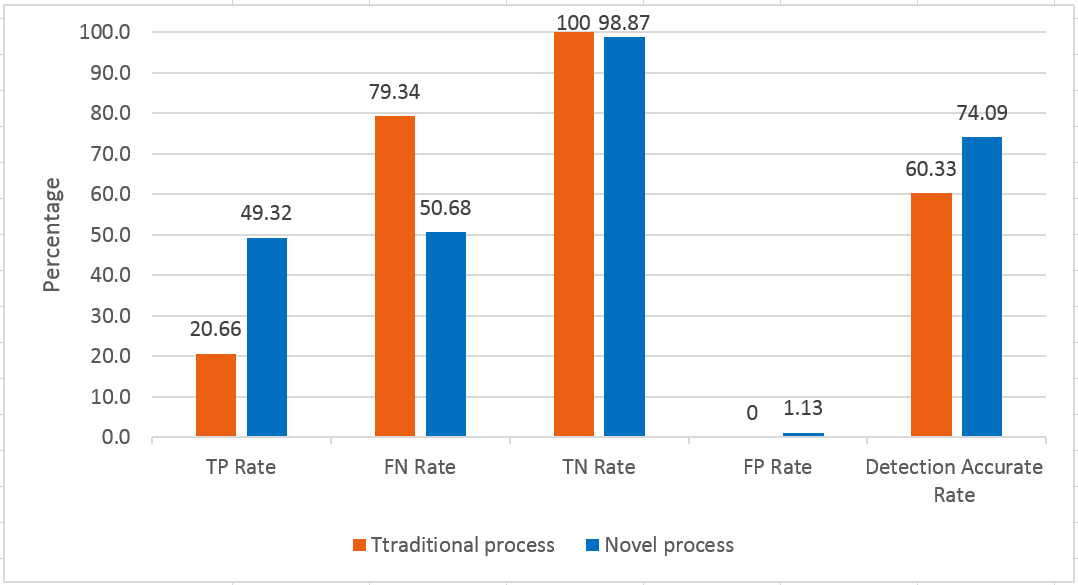
\includegraphics[width=1\textwidth]{images/results.jpg}
\caption{The results of the system performance analysis.}
\label{fig:graphresults}
\end{figure}

Table \ref{table_variableSysPerf} summarizes the notation for The System Performance Analysis.
The results obtained from the vehicle detection tests in three months is shown in Table \ref{table_vehiclesDetected}.
As a results, this novel process can detect 147 suspect vehicles more than the traditional process or equal to 138.68\% higher.
Fig. \ref{fig:graphresults} and Table \ref{table_results} show the results of the system performance analysis of the novel process that have the criminal or suspect vehicle detection rate is equal to 49.32\% and detection accurate rate is equal to 74.09\% which is an acceptable accurate rate. These results show that this technique can improve the detection capability of the suspect vehicle detection process.

\section{Discussion}
\label{sec:9}
The novel process still gain higher FP rate than the traditional process because using only color, brand and type of vehicles matching the blacklist can not separate the normal vehicles out of the target vehicles. However, we intend to improve the normal vehicle separation process by using the target vehicle data from Matching Score Module matching the vehicle database of Department of Land Transport (DLT), Thailand. If the target vehicle data do not match the DLT database, it is considered as the illegal vehicles and processed in the Vehicle Association with Criminal Activity Score Module. In addition, the use of the DLT database can improve the FN rate.

\section{Conclusion and Future Directions}
\label{sec:10}
This research proposes the use of vehicle reputation in couple with association analysis concept to improve the detection capability of suspect vehicle detection system.
The testing results from the previous section shows that the blacklist of criminal vehicles and criminal activity records obtained from criminal report database of DTI can be used to enhance the detection capability of suspect vehicle detection system and can address the limitations existing in the traditional process. 
In the future work, we plan to test this algorithm with the real scenario to compare with the formula in this research. 
In addition, we intend to explore the behavior of criminal vehicles crossing the checkpoint. This will allow us to analyze the crossing the checkpoint patterns of criminal vehicles and improve the suspect vehicle detection. Additionally, we intend to extend the suspect vehicle detection by using the vehicle crossing the checkpoint matching the vehicle database of DLT. This can be used to detect the illegal vehicles for reducing error of the normal vehicles detected as the suspect vehicles.

%\subsection{Subsection Heading}
%\label{sec:2}
%Your text goes here.

%\begin{equation}
%\vec{a}\times\vec{b}=\vec{c}
%\end{equation}

%\subsubsection{Subsubsection Heading}
%Your text goes here. Use the \LaTeX\ automatism for cross-references as
%well as for your citations, see Sect.~\ref{sec:1}.

%\paragraph{Paragraph Heading} %
%Your text goes here.

%\subparagraph{Subparagraph Heading.} Your text goes here.%
%
%\index{paragraph}
% Use the \index{} command to code your index words
%
% For tables use
%
%\begin{table}
%\centering
%\caption{Please write your table caption here}
%\label{tab:1}       % Give a unique label
%
% For LaTeX tables use
%
%\begin{tabular}{lll}
%\hline\noalign{\smallskip}
%first & second & third  \\
%\noalign{\smallskip}\hline\noalign{\smallskip}
%number & number & number \\
%number & number & number \\
%\noalign{\smallskip}\hline
%\end{tabular}
%\end{table}
%
%
% For figures use
%
%\begin{figure}
%\centering
% Use the relevant command for your figure-insertion program
% to insert the figure file.
% For example, with the option graphics use
%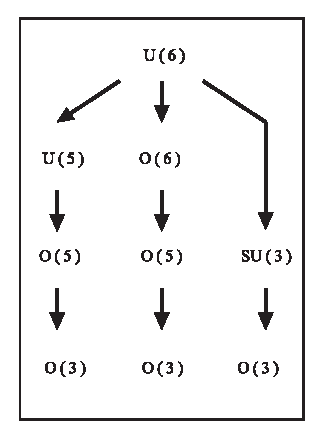
\includegraphics[height=4cm]{figure.eps}
%
% If not, use
%\picplace{5cm}{2cm} % Give the correct figure height and width in cm
%
%\caption{Please write your figure caption here}
%\label{fig:1}       % Give a unique label
%\end{figure}
%
% For built-in environments use
%
%\begin{theorem}
%Theorem text goes here.
%\end{theorem}
%
% or
%
%\begin{lemma}
%Lemma text goes here.
%\end{lemma}
%
%
% Problems or Exercises should be sorted chapterwise
%\section*{Problems}
%\addcontentsline{toc}{section}{Problems}
%
% Use the following environment.
% Don't forget to label each problem;
% the label is needed for the solutions' environment
%\begin{prob}
%\label{prob1}
%The problem\footnote{Footnote} is described here. The
%problem is described here. The problem is described here.
%\end{prob}

%\begin{prob}
%\label{prob2}
%\textbf{Problem Heading}\\
%(a) The first part of the problem is described here.\\
%(b) The second part of the problem is described here.
%\end{prob}



%

%%%%%%%%%%%%%%%%%%%%%% chapter.tex %%%%%%%%%%%%%%%%%%%%%%%%%%%%%%%%%
%
% sample chapter
%
% Use this file as a template for your own input.
%
%%%%%%%%%%%%%%%%%%%%%%%% Springer-Verlag %%%%%%%%%%%%%%%%%%%%%%%%%%

\chapter{Suspect Vehicle Detection using Vehicle Reputation with Association Analysis Concept}
\label{intro} % Always give a unique label
% use \chaptermark{}
% to alter or adjust the chapter heading in the running head

The suspect vehicle detection system normally compares the list of criminal license plates and vehicle license plates gathering from various sensors in order to identify the criminal vehicles or the suspect vehicles. 
However, the traditional process of comparing those license plates utilizing the matching of alphabet character is not effective. 
If the characters do not match any one character, the system can not detect the criminal vehicles or the suspect vehicles. 
This paper proposes the use of reputation algorithm to detect the criminal vehicles crossing the checkpoint whose license plates match the blacklist. 
In addition to that, we use association analysis concept to detect the suspect vehicles that have ever passed the checkpoint that may be related to the criminal activity records. 
Our method can detect the suspect vehicles with fake license plate by using color, brand and type of the vehicles instead of only the license plate matching to the blacklists.
These two techniques use a blacklist of criminal vehicles and criminal activity recorded in a criminal report database of Defence Technology Institute (DTI), Thailand, to help facilitate the detection process. 
The result shows that the reputation algorithm and the association analysis concept can improve the detection capability of the suspect vehicle detection system.

\section{Introduction}
\label{sec:1}
% Always give a unique label
% and use \ref{<label>} for cross-references
% and \cite{<label>} for bibliographic references
% use \sectionmark{}
% to alter or adjust the section heading in the running head
Reputation concept is a technique to classify object that commonly applied to various systems to make effective automatic detection, such as filtering email spam \cite{DBLP:taylor, lazzari}, vehicle classification \cite{ding,park}, ecommerce \cite{altman,page,resnick}, etc.
In addition, vehicle detection by only data classification process may be insufficient. Therefore, the association analysis process should be used together to increase the detection accuracy.
The traditional suspect vehicle detection process of comparing criminal license plates and vehicle license plates utilizing the matching of alphabet character is not effective. If the characters do not match any one character, the system can not detect criminal or suspect vehicles.

In this paper, we propose the approach using reputation concept to detect criminal vehicles crossing the checkpoint whose license plates match the blacklist. 
In addition, we use association analysis concept to detect the suspect vehicles which license plates do not match the blacklist, however this method uses color, brand and type of vehicles matching the blacklist to identify the vehicles that potentially involve in criminal activity.
The aim of this work is to improve the detection capability of suspect vehicle detection system.

In the next section, we discuss background information and previous studies using reputation algorithm and association analysis concept. Section III explains the research testbed and research design. Experimental results are shown in Section IV, and discussed in Section V. Section VI concludes and presents future directions.

\section{Literature Review}
\label{sec:2}

\subsection{Reputation Algorithm}
\label{sec:3}
The concept of reputation has been used to classify objects in a domain or community. 
An object with a higher reputation score gain more attraction than an object with a lower reputation score.  
Reputation concept has been applied to the several problems in vehicle scoring system.  
It works well for filtering false messages in vehicular ad hoc network (VANET) environments \cite{ding} and providing reliable reputation scores for vehicles in VANET initial deployment environment \cite{park}.
The reputation concept is also be applied to other practical applications. For example, Bradley Taylor \cite{DBLP:taylor} uses reputation to classify authenticated sender's domain as either spammy or not spammy within a large webmail service.  Reference \cite{altman} uses the axiomatic approach to deal PageRank, the most famous page ranking algorithm.
We propose the use of this concept to identify criminal vehicles that crossing the checkpoint. 
A high reputation score represents a criminal vehicle, whereas low reputation score represents a normal vehicle.

\subsection{Association Analysis Concept}
\label{sec:4}
Association analysis concept has been widely applied in various systems in previous research.
For example, the concept of mutual information have been used to estimate word association norms between words in English texts \cite{chruch} and to extract a triple of binary strings a, b, c \cite{romashchenko}.
Reference \cite{kaza} used association analysis by using the concept of mutual information measurement to identify potentially target vehicles that cross the border frequently with the vehicles which are involved in criminal activity.
Association analysis by using the idea of association rule has also been used to analyze frequent access crunode extracted from previous sequences \cite{li} and to extract valuable industrial data from massive data storage \cite{zhuang}.
G. Miao et al. \cite{miao} used a new ranking algorithm, based on Latent Association Analysis (LAA) by considering
the semantic associations among document pairs to rank target documents using the latent factor.

\section{Research Testbed and Design}
\label{sec:5}

\subsection{Research Testbed}
\label{sec:6}
The testbed for this research includes the blacklist of the criminal vehicle data set and the criminal activity data set obtained from criminal report database of Defence Technology Institute (DTI), Thailand.
Moreover, this testbed consists of the lists of the checkpoint crossing data set from various sensors includes the license plate, vehicle brand, vehicle color, vehicle type, checkpoint, crossing date and time. The checkpoint crossing data set is divided into two categories: 1) The one year records. 2) The real time checkpoint crossing records in three months. Details of these data sets are shown in Table \ref{table_inputData}.

\begin{table}[!t]
\renewcommand{\arraystretch}{1.2}
\caption{Summary of input data set}
\label{table_inputData}
\centering
\begin{tabular}{c|c}
\hline
\bfseries Input Data Set & \bfseries Summary\\
\hline
Number of the criminal vehicles in blacklist & 4801\\
\hline
Criminal activity records & 1972\\
\hline
The one year checkpoint crossing records & 992017\\
\hline
The real time checkpoint crossing records in three months & 281089\\
\hline
Number of the vehicles crossing the checkpoint in three months& 90563\\
\hline
Number of criminal vehicles crossing the checkpoint in three months& 513\\
\hline
\end{tabular}
\end{table}

\subsection{Research Design}
\label{sec:7}

\begin{figure*}
\centering
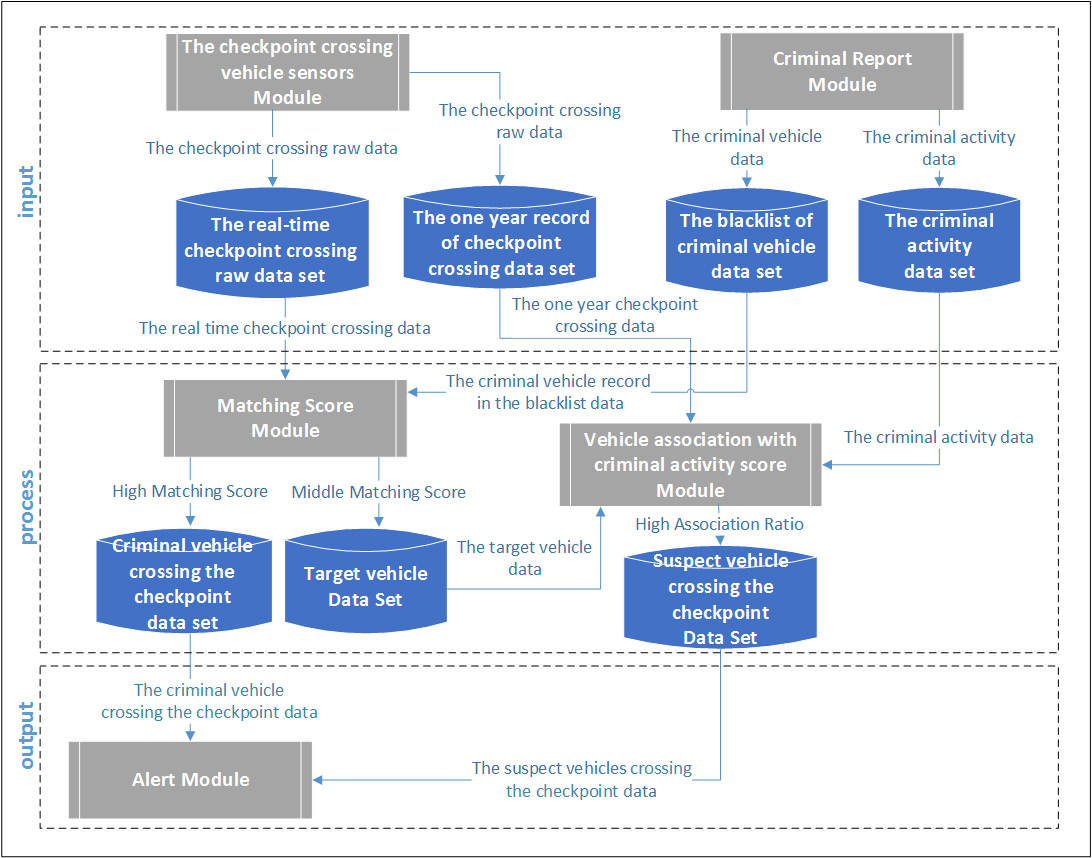
\includegraphics[width=1\textwidth]{images/myfigure.jpg}
\caption{Research design and process diagram.}
\label{fig:diagram}
\end{figure*}

Fig. \ref{fig:diagram} shows the research design and the evolution process of criminal or suspect vehicle detection at the checkpoint. This diagram is divided into three sections: 
1) Input section consists of the real time checkpoint crossing data set in three months, the one year records of checkpoint crossing data set, the blacklist of criminal vehicle data set, and criminal activity data set. 
2) Processing section consists of matching score module to detect the criminal vehicles that crossing the checkpoint and vehicle association with criminal activity score module to detect the suspect vehicles that crossing the checkpoint. In this research, we focus on the processing section shown in Fig.\ref{fig:diagram} which is explained in the following sub-sections. 
3) Output section serves as the alert of the criminal vehicle or suspect vehicle if the system detects the criminal vehicles or suspect vehicles that crossing the checkpoint. 

\subsubsection{Matching Score Module}
Matching Score Module is criminal vehicle detection process. 
First, we define attributes for classification and assign weight to each of the attributes. 
Higher weight is assigned to higher significant attributes.
In this research, we select the license plate, vehicle color, vehicle brand, and vehicle type to be used in the classification and we assign higher weight to license plate than vehicle color, vehicle brand, and vehicle type. 
The system compares the real time checkpoint crossing records in three months and criminal vehicle records in the blacklist by using following attributes: license plate, vehicle color, vehicle brand, and vehicle type. 
Subsequently, it computes the sum of all of the weighted attribute. 
The weighted sum is a single number to compare with the threshold.  
If weighted sum is greater than the high score threshold, referred to as “High Matching Score”, vehicle crossing the checkpoint will be considered as criminal vehicle and will be processed in the Alert Module. 
If weighted sum is less than the high score threshold and also greater than the low score threshold, referred to as “Middle Matching Score”, vehicle crossing the checkpoint will be considered as target vehicle and will be processed in the Vehicle Association with Criminal Activity Score Module. 

High Matching Score is calculated by the following attribute-matching condition: at least license plate matches with the blacklist.
Middle Matching Score is calculated by the following attribute-matching condition: vehicle color and vehicle brand and vehicle type match with the blacklist. 
Algorithm of Matching Score Module is shown in Fig. \ref{fig:matchingAlgo}. Table \ref{table_variableMatching} summarizes the notation for Matching Score Module.

\begin{figure}
\centering
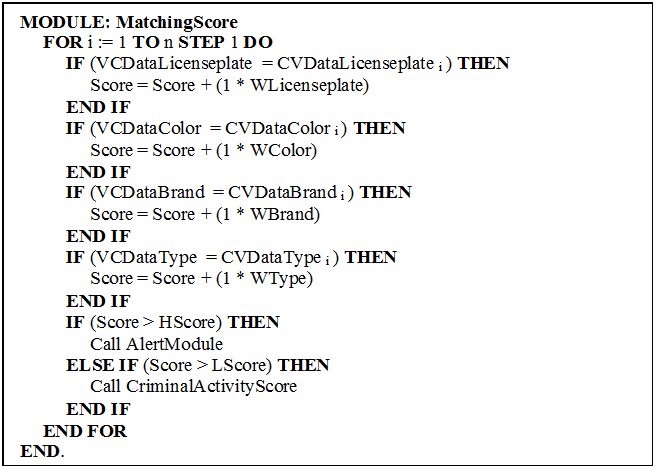
\includegraphics[width=1\textwidth]{images/MatchingAlgorithm.jpg}
\caption{Matching score module algorithm.}
\label{fig:matchingAlgo}
\end{figure}

%put these in Notation table
\begin{table}[!t]
\renewcommand{\arraystretch}{1.2}
\caption{Variable Description for Matching Score Module}
\label{table_variableMatching}
\centering
\begin{tabular}{c|l}
\hline
\bfseries Variables & \multicolumn{1}{c}{\bfseries Description}\\
\hline
VCDataLicenseplate & The license plate of vehicle that crossing the checkpoint.\\
\hline
VCDataColor & The color of vehicle that crossing the checkpoint.\\
\hline
VCDataBrand & The brand of vehicle that crossing the checkpoint.\\
\hline
VCDataType & The type of vehicle that crossing the checkpoint.\\
\hline
CVDataLicenseplate & The license plate of the criminal vehicle.\\
\hline
CVDataColor & The color of the criminal vehicle.\\
\hline
CVDataBrand & The brand of the criminal vehicle.\\
\hline
CVDataType & The type of the criminal vehicle.\\
\hline
WLicenseplate & The weight of license plate.\\
\hline
WColor & The weight of vehicle color.\\
\hline
WBrand & The weight of vehicle brand.\\
\hline
WType & The weight of vehicle type.\\
\hline
Score & The sum of all of the weighted attribute.\\
\hline
HScore & The high score threshold.\\
\hline
LScore & The low score threshold.\\
\hline
\end{tabular}
\end{table}

\subsubsection{Vehicle Association with Criminal Activity Score Module}
This module is a suspect vehicle detection process using association analysis concept to identify the vehicles that are potentially involved in criminal activities. 
We determine the number of all the one year checkpoint crossing lists of target vehicle by considering the matching of license plate, vehicle color, vehicle brand, and vehicle type. 
Consequently, we analyze the relationship between each of the criminal activity with all the one year checkpoint crossing records of target vehicle, and we further restricted the set to contain only checkpoint crossing records of target vehicle that already crossed the checkpoint near the location, date, and time of criminal activities. 
Such set can be indicated the number of involvement in criminal activities of target vehicle. 
Then we can calculated the association ratio by using in (1) by computing the fraction of number of involvement in criminal activities of target vehicle and number of the checkpoint crossing records of target vehicle to compare with the defined threshold.

\begin{eqnarray} 
\alpha \quad =\quad \frac { \nu  }{ \varsigma  }
\end{eqnarray}
where\mbox{ }\\
$\alpha$ = association ratio. \mbox{ }\\
$\nu$ = number of involvement in criminal activities of target vehicle.\mbox{ }\\
$\varsigma$ = total of the 1 year checkpoint crossing records of target vehicle.

If the vehicles with higher ratio than the threshold, they are considered potential suspect vehicles, and then the vehicle data will be processed in the Alert Module. 
Algorithm of Vehicle association with Criminal Activity Score Module is shown in Fig. \ref{fig:activityAlgo}. Table \ref{table_variableActivity} summarizes the notation for Vehicle Association with Criminal Activity Score Module.

\begin{figure}
\centering
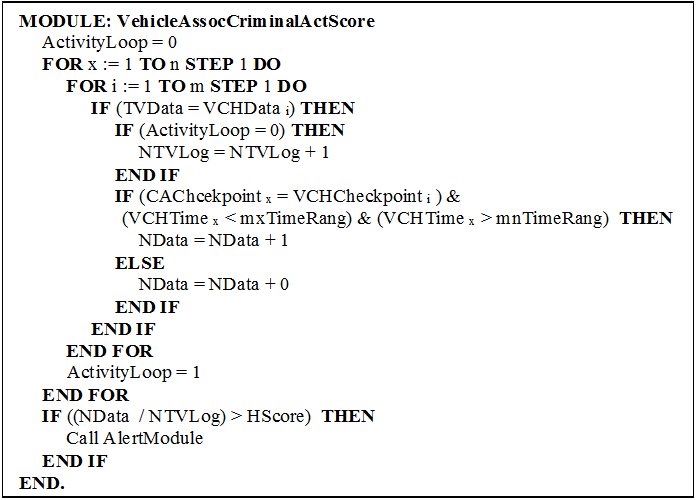
\includegraphics[width=1\textwidth]{images/activityAlgorithm2.jpg}
\caption{Vehicles association with criminal activity score module algorithm.}
\label{fig:activityAlgo}
\end{figure}

\begin{table}[!t]
\renewcommand{\arraystretch}{1.2}
\caption{Variable Description for Vehicle Association with Criminal Activity Score Module}
\label{table_variableActivity}
\centering
\begin{tabular}{c|l}
\hline
\bfseries The Variables & \multicolumn{1}{c}{\bfseries Description}\\
\hline
ActivityLoop & The variable that used to check first iteration in x loop.\\
\hline
TVData & The target vehicle data includes license plate, 
vehicle color, \\ & vehicle brand, and vehicle type.\\
\hline
VCHData & The one year record of checkpoint crossing data set includes  \\ & license plate, vehicle color, vehicle brand, and vehicle type.\\
\hline
NTVLog & Total of one year checkpoint crossing records of target vehicle.\\
\hline
CAChcekpoint & The checkpoint near the location of the criminal activity.\\
\hline
VCHCheckpoint & The checkpoint that target vehicle has ever passed.\\
\hline
VCHTime & Date and time of the checkpoint crossing record.\\
\hline
mxTimeRang & Date and time of the criminal activity plus 1 hour.\\
\hline
mnTimeRang & Date and time of the criminal activity minus 1 hour.\\
\hline
NData & Number of involvement in criminal activities of target vehicle.\\
\hline
HScore & The defined threshold.\\
\hline
\end{tabular}
\end{table}

\section{Experimental Results}
\label{sec:8}
To analyze system performance, there are four factors for analysis as follows:
1) True positive (TP) is the number of the criminal and suspect vehicles that are analyzed as the criminal and suspect vehicles.  
2) True negative (TN) is the number of the normal vehicles that are analyzed as the normal vehicles. 
3) False positive (FP) is the number of the normal vehicles that are analyzed as the criminal and suspect vehicles. 
4) False negative (FN) is the number of the criminal and suspect vehicles that are analyzed as the normal vehicles. 
Such factors can be calculated by using this formula:\\
$$ \text{TP Rate} =  \frac{\text{NofCSVDetectedAsCSV}}{\text{TofCSV}} $$\\
$$ \text{FN Rate} =  \frac{\text{NofCSVDetectedAsNV}}{\text{TofCSV}} $$\\
$$ \text{TN Rate} =  \frac{\text{NofNVDetectedAsNV}}{\text{TofNV}} $$\\ 
$$ \text{FP Rate} =  \frac{\text{NofNVDetectedAsCSV}}{\text{TofNV}} $$\\
$$ \text{Detection Accurate Rate} =  \frac{\text{TP Rate + TN Rate}}{\text{2}} $$

%put this in Notation
\begin{table}[!t]
\renewcommand{\arraystretch}{1.2}
\caption{Variable Description for The System Performance Analysis}
\label{table_variableSysPerf}
\centering
\begin{tabular}{c|l}
\hline
\bfseries Variables & \multicolumn{1}{c}{\bfseries Description}\\
\hline
NofCSVDetectedAsCSV & The number of the criminal and suspect vehicles that \\ & are detected as the criminal and suspect vehicle.\\
\hline
TofCSV & The total of all the criminal and suspect vehicles.\\
\hline
NofCSVDetectedAsNV & The number of the criminal and suspect vehicles that \\ & are detected as the normal vehicle.\\
\hline
NofNVDetectedAsNV & The number of the normal vehicles that are detected \\ & as the normal vehicle.\\
\hline
TofNV & The total of all the normal vehicles.\\
\hline
NofNVDetectedAsCSV & The number of the normal vehicles that are detected \\ & as the criminal and suspect vehicle.\\
\hline
\end{tabular}
\end{table}

\begin{table}[!t]
\renewcommand{\arraystretch}{1.2}
\caption{summary of the vehicles detected in three months}
\label{table_vehiclesDetected}
\centering
\begin{tabular}{c|c|c}
\hline
\bfseries Vehicle Detection & \bfseries Traditional process & \bfseries Novel process\\
\hline
Criminal Vehicles & 106 & 106\\
\hline
Suspect Vehicles & 0 & 147\\
\hline
\end{tabular}
\end{table}

\begin{table}[!t]
\renewcommand{\arraystretch}{1.2}
\caption{The Results of The System Performance Analysis}
\label{table_results}
\centering
\begin{tabular}{c|c|c}
\hline
\bfseries Analysis Rate & \bfseries Traditional process & \bfseries Novel process\\
\hline
TP Rate & 20.66\% & 49.32\%\\
\hline
FN Rate & 79.34\% & 50.68\%\\
\hline
TN Rate & 100\% & 98.87\%\\
\hline
FP Rate & 0\% & 1.13\%\\
\hline
Detection Accurate Rate & 60.33\% & 74.09\%\\
\hline
\end{tabular}
\end{table}

\begin{figure}
\centering
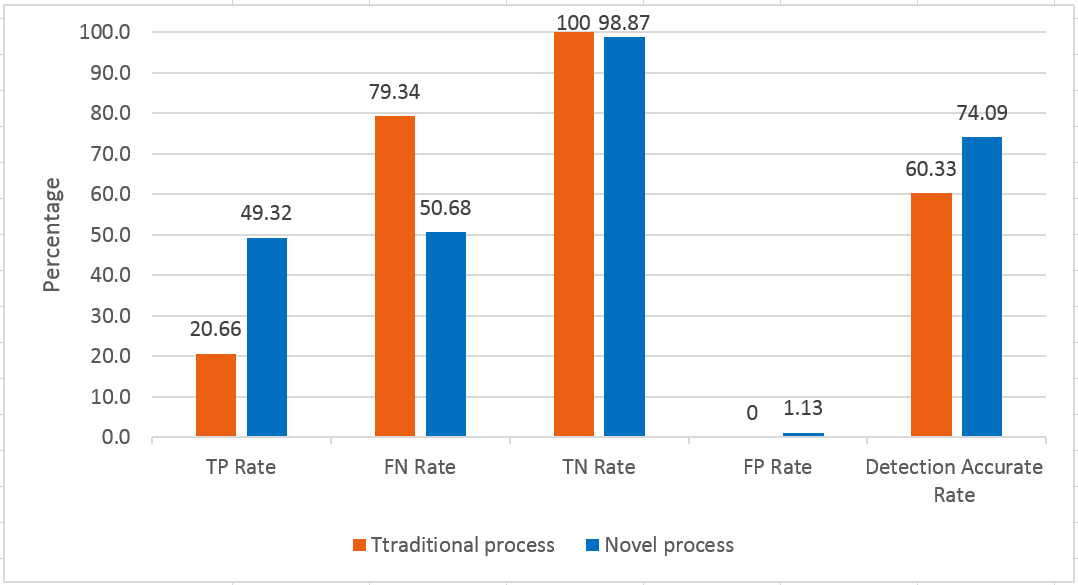
\includegraphics[width=1\textwidth]{images/results.jpg}
\caption{The results of the system performance analysis.}
\label{fig:graphresults}
\end{figure}

Table \ref{table_variableSysPerf} summarizes the notation for The System Performance Analysis.
The results obtained from the vehicle detection tests in three months is shown in Table \ref{table_vehiclesDetected}.
As a results, this novel process can detect 147 suspect vehicles more than the traditional process or equal to 138.68\% higher.
Fig. \ref{fig:graphresults} and Table \ref{table_results} show the results of the system performance analysis of the novel process that have the criminal or suspect vehicle detection rate is equal to 49.32\% and detection accurate rate is equal to 74.09\% which is an acceptable accurate rate. These results show that this technique can improve the detection capability of the suspect vehicle detection process.

\section{Discussion}
\label{sec:9}
The novel process still gain higher FP rate than the traditional process because using only color, brand and type of vehicles matching the blacklist can not separate the normal vehicles out of the target vehicles. However, we intend to improve the normal vehicle separation process by using the target vehicle data from Matching Score Module matching the vehicle database of Department of Land Transport (DLT), Thailand. If the target vehicle data do not match the DLT database, it is considered as the illegal vehicles and processed in the Vehicle Association with Criminal Activity Score Module. In addition, the use of the DLT database can improve the FN rate.

\section{Conclusion and Future Directions}
\label{sec:10}
This research proposes the use of vehicle reputation in couple with association analysis concept to improve the detection capability of suspect vehicle detection system.
The testing results from the previous section shows that the blacklist of criminal vehicles and criminal activity records obtained from criminal report database of DTI can be used to enhance the detection capability of suspect vehicle detection system and can address the limitations existing in the traditional process. 
In the future work, we plan to test this algorithm with the real scenario to compare with the formula in this research. 
In addition, we intend to explore the behavior of criminal vehicles crossing the checkpoint. This will allow us to analyze the crossing the checkpoint patterns of criminal vehicles and improve the suspect vehicle detection. Additionally, we intend to extend the suspect vehicle detection by using the vehicle crossing the checkpoint matching the vehicle database of DLT. This can be used to detect the illegal vehicles for reducing error of the normal vehicles detected as the suspect vehicles.

%\subsection{Subsection Heading}
%\label{sec:2}
%Your text goes here.

%\begin{equation}
%\vec{a}\times\vec{b}=\vec{c}
%\end{equation}

%\subsubsection{Subsubsection Heading}
%Your text goes here. Use the \LaTeX\ automatism for cross-references as
%well as for your citations, see Sect.~\ref{sec:1}.

%\paragraph{Paragraph Heading} %
%Your text goes here.

%\subparagraph{Subparagraph Heading.} Your text goes here.%
%
%\index{paragraph}
% Use the \index{} command to code your index words
%
% For tables use
%
%\begin{table}
%\centering
%\caption{Please write your table caption here}
%\label{tab:1}       % Give a unique label
%
% For LaTeX tables use
%
%\begin{tabular}{lll}
%\hline\noalign{\smallskip}
%first & second & third  \\
%\noalign{\smallskip}\hline\noalign{\smallskip}
%number & number & number \\
%number & number & number \\
%\noalign{\smallskip}\hline
%\end{tabular}
%\end{table}
%
%
% For figures use
%
%\begin{figure}
%\centering
% Use the relevant command for your figure-insertion program
% to insert the figure file.
% For example, with the option graphics use
%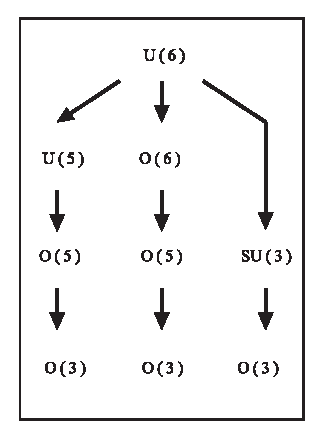
\includegraphics[height=4cm]{figure.eps}
%
% If not, use
%\picplace{5cm}{2cm} % Give the correct figure height and width in cm
%
%\caption{Please write your figure caption here}
%\label{fig:1}       % Give a unique label
%\end{figure}
%
% For built-in environments use
%
%\begin{theorem}
%Theorem text goes here.
%\end{theorem}
%
% or
%
%\begin{lemma}
%Lemma text goes here.
%\end{lemma}
%
%
% Problems or Exercises should be sorted chapterwise
%\section*{Problems}
%\addcontentsline{toc}{section}{Problems}
%
% Use the following environment.
% Don't forget to label each problem;
% the label is needed for the solutions' environment
%\begin{prob}
%\label{prob1}
%The problem\footnote{Footnote} is described here. The
%problem is described here. The problem is described here.
%\end{prob}

%\begin{prob}
%\label{prob2}
%\textbf{Problem Heading}\\
%(a) The first part of the problem is described here.\\
%(b) The second part of the problem is described here.
%\end{prob}



%

%\appendix
%\include{appendix}

\backmatter%%%%%%%%%%%%%%%%%%%%%%%%%%%%%%%%%%%%%%%%%%%%%%%%%%%%%%%

\chapter*{Solutions}
\addcontentsline{toc}{chapter}{Solutions}
\markboth{Solutions}{Solutions}

\section*{Problems of Chapter~\ref{intro}}

\begin{sol}{prob1}
The solution is revealed here.
\end{sol}


\begin{sol}{prob2}
\textbf{Problem Heading}\\
(a) The solution of first part is revealed here.\\
(b) The solution of second part is revealed here.
\end{sol}


%%%%%%%%%%%%%%%%%%%%%%%% referenc.tex %%%%%%%%%%%%%%%%%%%%%%%%%%%%%%
% sample references
% "computer science"
%
% Use this file as a template for your own input.
%
%%%%%%%%%%%%%%%%%%%%%%%% Springer-Verlag %%%%%%%%%%%%%%%%%%%%%%%%%%

%
% BibTeX users please use
% \bibliographystyle{}
% \bibliography{}
%
% Non-BibTeX users please use
\begin{thebibliography}{99.}
%
% and use \bibitem to create references.
%
% Use the following syntax and markup for your references
%
% Monographs

% Start Bon Custom
\bibitem{DBLP:taylor} B. Taylor, “Sender reputation in a large webmail service,” in CEAS, 2006.

\bibitem{lazzari} L. Lazzari, M. Mari, and A. Poggi, “A collaborative and multi-agent system for e-mail filtering and classification,” in Collaborative Computing: Networking, Applications and Worksharing, 2005 International Conference on, 2005, pp. 8 pp.–

\bibitem{ding} Q. Ding, X. Li, M. Jiang, and X. Zhou, “Reputation management in vehicular ad hoc networks,” in Multimedia Technology (ICMT), 2010 International Conference on, Oct 2010, pp. 1–5.

\bibitem{park} S. Park, B. Aslam, and C. Zou, “Long-term reputation system for vehicular networking based on vehicle’s daily commute routine,” in Consumer Communications and Networking Conference (CCNC), 2011 IEEE, Jan 2011, pp. 436–441.

\bibitem{altman} A. Altman and M. Tennenholtz, “Ranking systems: The pagerank axioms,” in Proceedings of the 6th ACM Conference on Electronic Commerce, ser. EC ’05. New York, NY, USA: ACM, 2005, pp. 1–8. [Online]. Available: http://doi.acm.org/10.1145/1064009.1064010

\bibitem{page} L. Page, S. Brin, R. Motwani, and T. Winograd, “The pagerank citation ranking: Bringing order to the web,” in Proceedings of the 7th International World Wide Web Conference, Brisbane, Australia, 1998, pp. 161–172. [Online]. Available: citeseer.nj.nec.com/page98pagerank.html

\bibitem{resnick} P. Resnick and R. Zeckhauser, “Trust among strangers in Internet transactions: Empirical analysis of eBay’s reputation system,” in The Economics of the Internet and E-Commerce, ser. Advances in Applied Microeconomics, M. R. Baye, Ed. Elsevier Science, 2002, vol. 11, pp. 127–157. [Online]. Available: http://www.si.umich.edu/ presnick/papers/ebayNBER/index.html

\bibitem{chruch} K. W. Church and P. Hanks, “Word association norms, mutual information, and lexicography,” Comput. Linguist., vol. 16, no. 1, pp. 22–29, Mar. 1990. [Online]. Available: http://dl.acm.org/citation.cfm?id=89086.89095

\bibitem{romashchenko} A. Romashchenko, “Extracting the mutual information for a triple of binary strings,” in Computational Complexity, 2003. Proceedings. 18th IEEE Annual Conference on, July 2003, pp. 221–229.

\bibitem{kaza} S. Kaza, T.Wang, H. Gowda, and H. Chen, “Target vehicle identification for border safety using mutual information,” in Intelligent Transportation Systems, 2005. Proceedings. 2005 IEEE, Sept 2005, pp. 1141–1146.

\bibitem{li} L. Xiang-wei and Z. Shuang-ping, “A novel web authoritative page mining algorithm based on association analysis,” in Knowledge Acquisition and Modeling (KAM), 2011 Fourth International Symposium on, Oct 2011, pp. 136–138.

\bibitem{zhuang} Z. Zhuang and B. Zhang, “Application of association analysis in digital content industry,” in Computational Intelligence and Design (ISCID), 2012 Fifth International Symposium on, vol. 1, Oct 2012, pp. 18–21.

\bibitem{miao} G. Miao, Z. Guan, L. E. Moser, X. Yan, S. Tao, N. Anerousis, and J. Sun, “Latent association analysis of document pairs,” in Proceedings of the 18th ACM SIGKDD International Conference on Knowledge Discovery and Data Mining, ser. KDD ’12. New York, NY, USA: ACM, 2012, pp. 1415–1423. [Online]. Available: http://doi.acm.org/10.1145/2339530.2339752

% End Bon Custom

%\bibitem{monograph} Kajan E (2002)
%Information technology encyclopedia and acronyms. Springer, Berlin
%Heidelberg New York

% Contributed Works
%\bibitem{contribution} Broy M (2002) Software engineering -- From
%auxiliary to key technologies. In: Broy M, Denert E (eds)
%Software Pioneers. Springer, Berlin Heidelberg New York

% Journal
%\bibitem{journal} Che M, Grellmann W, Seidler S (1997)
%Appl Polym Sci 64:1079--1090

% Theses
%\bibitem{thesis} Ross DW (1977) Lysosomes and storage diseases. MA
%Thesis, Columbia University, New York

\end{thebibliography}

\printindex

%%%%%%%%%%%%%%%%%%%%%%%%%%%%%%%%%%%%%%%%%%%%%%%%%%%%%%%%%%%%%%%%%%%%%%

\end{document}





